\documentclass{article}
\usepackage{graphicx}


% if you need to pass options to natbib, use, e.g.:
%     \PassOptionsToPackage{numbers, compress}{natbib}
% before loading neurips_2024


% ready for submission
\usepackage{neurips_2024}
\usepackage{algorithm}
\usepackage{algorithmic}
\usepackage{xcolor}
\usepackage{subfigure}
\usepackage{amsmath}
\usepackage{autobreak}
%\usepackage[lined,boxed,commentsnumbered]{algorithm2e}
\usepackage{multirow}
\usepackage{fontawesome}
\allowdisplaybreaks

% to compile a preprint version, e.g., for submission to arXiv, add add the
% [preprint] option:
%     \usepackage[preprint]{neurips_2024}


% to compile a camera-ready version, add the [final] option, e.g.:
%     \usepackage[final]{neurips_2024}


% to avoid loading the natbib package, add option nonatbib:
%    \usepackage[nonatbib]{neurips_2024}


\usepackage[utf8]{inputenc} % allow utf-8 input
\usepackage[T1]{fontenc}    % use 8-bit T1 fonts
\usepackage{hyperref}       % hyperlinks
\usepackage{url}            % simple URL typesetting
\usepackage{booktabs}       % professional-quality tables
\usepackage{amsfonts}       % blackboard math symbols
\usepackage{nicefrac}       % compact symbols for 1/2, etc.
\usepackage{microtype}      % microtypography
\usepackage{xcolor}         % colors
\usepackage{natbib}

% -------------------------允许算法跨页-------------
\usepackage{lipsum}

\makeatletter
\newenvironment{breakablealgorithm}
  {% \begin{breakablealgorithm}
   \begin{center}
     \refstepcounter{algorithm}% New algorithm
     \hrule height.8pt depth0pt \kern2pt% \@fs@pre for \@fs@ruled
     \renewcommand{\caption}[2][\relax]{% Make a new \caption
       {\raggedright\textbf{\ALG@name~\thealgorithm} ##2\par}%
       \ifx\relax##1\relax % #1 is \relax
         \addcontentsline{loa}{algorithm}{\protect\numberline{\thealgorithm}##2}%
       \else % #1 is not \relax
         \addcontentsline{loa}{algorithm}{\protect\numberline{\thealgorithm}##1}%
       \fi
       \kern2pt\hrule\kern2pt
     }
  }{% \end{breakablealgorithm}
     \kern2pt\hrule\relax % \@fs@post for \@fs@ruled
   \end{center}
  }
\makeatother

\makeatletter
\newcommand\multiline[1]{\parbox[t]{\dimexpr\linewidth-\ALG@thistlm}{#1}}
\makeatother
\title{Toward Stealthy and Powerful Clean-label Backdoor Attacks via Trigger-specific Selection of Samples}


% The \author macro works with any number of authors. There are two commands
% used to separate the names and addresses of multiple authors: \And and \AND.
%
% Using \And between authors leaves it to LaTeX to determine where to break the
% lines. Using \AND forces a line break at that point. So, if LaTeX puts 3 of 4
% authors names on the first line, and the last on the second line, try using
% \AND instead of \And before the third author name.


\author{%
  David S.~Hippocampus\thanks{Use footnote for providing further information
    about author (webpage, alternative address)---\emph{not} for acknowledging
    funding agencies.} \\
  Department of Computer Science\\
  Cranberry-Lemon University\\
  Pittsburgh, PA 15213 \\
  \texttt{hippo@cs.cranberry-lemon.edu} \\
  % examples of more authors
  % \And
  % Coauthor \\
  % Affiliation \\
  % Address \\
  % \texttt{email} \\
  % \AND
  % Coauthor \\
  % Affiliation \\
  % Address \\
  % \texttt{email} \\
  % \And
  % Coauthor \\
  % Affiliation \\
  % Address \\
  % \texttt{email} \\
  % \And
  % Coauthor \\
  % Affiliation \\
  % Address \\
  % \texttt{email} \\
}


\begin{document}


\maketitle


\begin{abstract}
Backdoor attacks aim to covertly inject attacker-desired behavior into Deep Neural Networks (DNNs). Clean-label backdoor attacks are seen as the stealthiest attacks as adversaries can only poison samples from the target class without changing their labels. The effectiveness of clean-label attacks can be enhanced by carefully selecting poisoned samples. However, the collaborative effect of data poisoning selection and trigger design remains under-explored. In this paper, we highlight the significance of trigger-specific sample selection from two angles: boosting trigger stealthiness and efficiency. Firstly, we enhance the Bits Per Pixel (BPP) trigger by distinct color quantitation based on the human eyes' inherent poor insensitivity to blue light, and the invisibility of the trigger is ensured by poisoning the images with the smallest perceived distance changes during quantization. By poisoning 2.5\% images of CIFAR10, the optimized attack overwhelms the BPP Attack by Attack Success Rate (ASR) from 12.5\% to 68.89\% even without label poisoning and training control. Secondly, we notice that current metrics ignore the competition between trigger features and non-target class robust features. For example, the forgetting-event metric only focuses on the frequency of forgetting events without paying attention to the category information of incorrect results. In sample selection, the consideration of category information for incorrect results varies across diverse triggers due to different extent of interference from non-target features on the learning of toxic features. Extensive experiments exhibit the tremendous superiority of trigger-specific metrics upon enhancing attacks across CIFAR10, CIFAR100, and Tiny-imagenet datasets. 
\end{abstract}

\paragraph{Remark of poisoned samples generation}
The effectiveness of poison-only backdoor attacks hinges on the selection of poisoned data and the design of the trigger. However, \textbf{sample selection and trigger design of current methods are handled independently.} The goal of our paper is to find a simple but efficient poisoning sample selection strategy that can be generally applicable to various poison-only clean-label backdoor attacks by exploring the collaborative effect of step 1 and step 2. %优化abstract,强调方法的泛化性,简写Bppattack

\section{Introduction}
Deep neural networks (DNNs) have gained widespread adoption owing to their proven effectiveness and efficiency. However, their accuracy comes at the cost of intelligibility: it is usually unclear how they make their decisions (\citet{radenovic2022neural}) and what they have learned, which poses significant challenges for scientists in efficiently defending the backdoor attacks (\citet{doan2021backdoor},\citet{287378}, \citet{10.1145/3576915.3616617}). The deployment of models harboring security flaws pose a threat to the development of secure applications in important areas like finance, healthcare, Machine-Learning-as-a-Service (MLaaS)(\citet{huang2024uba}), autonomous driving, and beyond, thus rendering the investigation of backdoor attacks a vital area of research endeavor. 

Backdoor attacks aim to inject the behavior desired by the attacker into the model in a covert manner. A successful covert attack hinges on choosing a trigger pattern that remains effective at low poisoning rates while being stealthy to the human eye to evade manual inspections. Furthermore, most attacks can be set up as more challenging clean-label attack scenarios. Clean-label backdoor attacks ((\citet{huynh2024combat}, \citet{zhao2024exploring})) are seen as the stealthiest attacks as adversaries can only poison samples from the target class without changing their labels. However, current attacks confront challenges in achieving both potency and invisibility without label poisoning in a straightforward way. For example, \citet{wang2022bppattack} proposed BppAttack, a stealthy attack which induces triggers based on image quantization and dithering. Due to the limited potency of imperceptible alterations, adversaries resort to adversarial training with label flipping to effectively embed the triggers. Generally speaking, BppAttack cannot achieve a powerful clean-label invisible backdoor attack by only poisoning the dataset.

\citet{gao2023not} reveals that the challenge of clean-label attacks primarily stems from the conflicting effects of 'robust features' associated with the target class within poisoned samples.  Therefore, a simple yet effective plug-in method is proposed to enhance clean-label backdoor attacks by poisoning ‘hard’ instead of random samples. However, existing methods (\citet{hayase2022few}, \citet{li2023explore}, \citet{li2024proxy}, \citet{hungwicked}, \citet{wang2025not}, \citet{han2024backdooring}) overlook the stealthiness aspect of poisoned data selection and fail to consider the influence of non-target class robust features on trigger feature learning. The collaborative effect of data poisoning selection and trigger design remains under-explored. In this paper, we highlight the significance of trigger-specific sample selection in augmenting both trigger stealthiness and efficiency.

First of all, we demonstrate how to effectively and simply address the dilemma of the BppAttack by designing a trigger-specific sample selection strategy from the perspective of stealthiness. Computers represent image colors based on the three primary colors and BppAttack quantizes three colors uniformly (32:32:32), neglecting the differences in human visual perception and machine representation. For machine learning models, the data from these three color channels are treated equally during training. However, human perception exhibits marked differences in sensitivity to different colors. For example, humans exhibit limited sensitivity to blue light because the blue-sensitive cone cells comprises merely 5\% in the human visual system. \citet{land1971lightness} sets the ratio of RGB as 60:35:6 from the perspective of human perception. Therefore, we adjusted the quantization ratios of the three colors, with particular emphasis on increasing the poisoning intensity in the blue channel. It is worth noting that human eye's sensitivity to color perception is complex, with variations across different lighting scenarios and among individuals. Therefore, additional measures are still needed to ensure the invisibility of the trigger. The stealthiness of the optimized trigger, dubbed Multi-BPP, is assured in this paper by poisoning the images with the smallest perceived distance variations during quantization. Compared to BppAttack, Multi-BPP increases Attack Success Rate (ASR) from 12.5\% to 68.89\% with 2.5\% poison rate in CIFAR10 without label flipping and training control in a straightforward approach.

Furthermore, trigger-specific sample selection demonstrates significant advantages in further enhancing the efficiency of backdoor attacks.  Current trigger-uncoupled metrics (forgetting events, loss, and gradients) ignore the competition between trigger features and non-target class robust features. For example, current methods based on forgetting events (\citet{gao2023not}) only focuses on the frequency of forgetting events without paying attention to the category information of incorrect results. Extensive experiments on the CIFAR10, CIFAR100, and Tiny-ImageNet datasets indicate that the optimal balance between the diversity of jumped categories and the frequency of forgetting depends on the trigger pattern. Most triggers can be classified into two categories based on the size of the poisoning area. Backdoor attacks, represented by Badnets (\citet{gu2017badnets}), use visible embedding high-intensity features in a limited section of images as triggers. A small but high-intensity poisoning area allows the model to learn trigger features with minimal interference from global features (robust features of non-target classes) as models tend to take shortcuts during training. Alternatively, other attacks including blend (\citet{chen2017targeted}) enhance the stealthiness of the triggers while maintaining a high attack success rate by contaminating the entire image, which is the most classical trigger pattern having the widest room for design. The competition between trigger features and non-target class robust features matters when devising sample selection to enhance the efficiency of those triggers. For diverse triggers, the extent to which category information of incorrect results is considered varies in sample selection. Compared to existing trigger-decoupled methods, an apt trigger-specific sample selection can markedly enhance the attack success rate (ASR) of clean-label backdoor attacks.

The contributions of our paper are as follows:

\begin{itemize}
\item Compared to BppAttack (\citet{wang2022bppattack}), the proposed Multi-BPP increases Attack Success Rate (ASR) from 12.5\% to 68.89\% with 2.5\% poison rate in CIFAR10 without label flipping and training control by simply designing a trigger-specific sample selection strategy from the perspective of stealthiness. 
\item The trigger-specific metrics, optimized by accounting for the competition between trigger features and robust features of non-target classes, exhibit tremendous superiority in enhancing attacks across CIFAR10, CIFAR100, and Tiny-imagenet datasets. It is worth noting that, given that backdoor defense usually assumes that the poisonous features are the strongest features in the training data (\citet{khaddaj2023rethinking}), attacks by poisoning the overall region gradually become the main research direction of backdoor attacks due to concealment and feature strength control. Therefore, robust features of non-target classes play an especially important role for most advanced attacks.
\item The efficiency of poison-only attacks depends on the sample selection and the trigger pattern. However, the collaborative effect of data poisoning selection and trigger design remains under-explored. In our paper, extensive experiments demonstrate the value to construct stealthy and powerful clean-label backdoor attacks via trigger-specific selection of samples.
\end{itemize}

\section{Related Work}
Deep neural networks (DDNs) are vulnerable to backdoor attacks. The trojaned models function normally with regular inputs but misclassify to a target label with input stamped by the trigger (\citet{gu2017badnets}, \citet{chen2017targeted}). At present, attackers have designed effective backdoor attacks in multimodal learning (\citet{wang2024invisible}, \citet{han2024backdooring}), federated learning (\citet{li20233dfed}, \citet{chen2023practical}), diffusion model (\citet{chou2023villandiffusion}, \citet{li2024invisible}), dataset distillation (\citet{liu2023backdoor}) and other scenarios (\citet{zhao2024exploring}). Furthermore, attackers explore various ways to inject the desired behavior into DDNs. \citet{bai2022hardly} construct attack by manipulating model parameters (\citet{qi2022towards}) via bit flipping. UBA-Inf (\citet{huang2024uba}) activates a camouflaged backdoor through unlearning requests.

Despite the variety of application scenarios and triggering methods for backdoor attacks, mainstream research predominantly focuses on Computer Vision (CV), given its widespread use. Notably, data-poisoning backdoor attacks have attracted significant attention owing to their practicality. These attacks aim to embed backdoors into models by manipulating the training dataset, without controlling the training process of the target model. The effectiveness of a data poisoning attack depends on the design of the trigger and the selection of poisoned data. However, \textbf{current related research is conducted independently and the synergistic effect has not been adequately emphasized.}
\subsection{Trigger Design}
Traditional attacks (\citet{gu2017badnets}, \citet{chen2017targeted}) utilize visible patch-based triggers (e.g., a square pattern), rendering them detectable by both humans and machines. The essence of advanced trigger design lies in identifying a stealthy feature that is conducive to machine learning. 

In computer vision (CV) applications, the common strategy involves incorporating minor perturbations by tweaking the pixel values and positions of the original image (\citet{bai2022hardly}). Despite its inherent stealthiness, the constraint of invisibility poses a significant limitation and conflict in balancing attack efficiency and the utility of the poisoned model. Efforts to overcome these challenges frequently result in high injection rates, ineffective backdoor embeddings, limited transferability, and/or weakened robustness. For example, \citet{wang2022bppattack} introduces BppAttack, a covert attack mechanism that leverages image quantization and dithering to induce triggers. Given the constrained effectiveness of imperceptible modifications, adversaries struggle to enhance the efficiency of attacks by employing adversarial training combined with label flipping. 

To overcome the conflict between effectiveness and stealthiness, \citet{gao2024backdoor} generates powerful and stealthy triggers by viewing trigger design as a bi-level optimization problem. Additionally, \citet{wenger2022finding} introduces natural triggers based on the hypothesis that there may be naturally occurring physically colocated objects already present in popular datasets such as ImageNet. Furthermore, \citet{lin2020composite} propose a Trojan trigger formulated from a combination of existing benign features to bypass the machine detection.
\paragraph{Summary}
 Although designing a powerful trigger is essential, these methods often fail to benefit other backdoor attacks accordingly. It is not feasible to simply combine existing methods to design an effective sparse and invisible backdoor attack. In the clean-label setting, approaches that rely solely on complex trigger designs (\citet{wang2024invisible}, \citet{huynh2024combat}) to ensure attack effectiveness are gradually encountering bottlenecks. Therefore, \textbf{seeking breakthroughs from a holistic perspective of the attack is an important issue.}
\subsection{Sample Selection}
Lowering the percentage of poisoned samples is one of the most direct ways to increase the stealthiness of backdoor attacks. Clean-label backdoor attacks are seen as the stealthiest attacks as adversaries can only poison samples from the target class without changing their labels. The effectiveness of clean-label attacks can be enhanced by carefully selecting poisoned samples. \citet{gao2023not} reveals the varying importance of each poisoning sample and selects 'hard' samples based on three metrics (e.g., forgetting events, gradients, and loss). \citet{han2024backdooring} further improves the efficiency of attacks based on optimized backdoor gradient-based score (BAGS). Moreover, \citet{hayase2022few} poses sample selection as a bi-level optimization problem: construct strong poison examples that maximize the attack success rate (ASR). Furthermore, some scientists propose novel sample selection methods based on poisoning masks (\citet{zhu2023boosting}), confidence-based scoring (\citet{wu2023computation}), and high-frequency energy (\citet{xun2024minimalism}). 
\paragraph{Summary}
Current research on sample selection focuses on designing new metrics or training derivations to construct data-efficiency attacks without recognizing the synergistic effect between triggers and sample selection. BppAttack draws our attention to the fact that there are few invisible attacks without training trigger generators. We demonstrate how to effectively overcome the dilemma of BppAttack based on a trigger-specific sample selection without extra training from the perspective of stealthiness. Meanwhile, current methods overlook the differential interference of category information under different trigger feature learning. Therefore, from the perspective of enhancing attack effectiveness, trigger-specific sample selection is a valuable research direction.
\section{Methodology}
\subsection{Preliminaries}
\subsubsection{Model Training}
The model output function of the image classification can be denoted by \(f_\theta:X \to Y\), where \(x \in X=\{0,1,\ldots,255\}^{C \times H \times W }\) represents an image domain, \(Y=\{y_1,y_2,\ldots,y_k\}\) is a set of k classes, and \(\theta\) denotes the parameters that a DNN learned form the begin training dataset \(D_{tr} = \{(x_i, y_i)\}_{i=1}^{N}\). 

The benign training with \(D_{tr}\) can be seen as a single-level optimization problem. The optimization seeks a model \(f_\theta\) by solving the following problem during training:
\begin{equation}
\min_{\theta} L(D_{tr}, f_{\theta}) = \sum_{i=1}^{N_{tr}}l(x_i,y_i,f_{\theta}),
\end{equation}
where \(l\) is the loss function (e.g., the cross-entropy), and \((x_i,y_i) \in D_{tr}\).
\subsubsection{Poion-only Clean-label Backdoor Attacks}
\paragraph{Attack Knowledge}
In a poison-only backdoor attack, an adversary has access to the original training dataset \(D_{tr}\) and is allowed to inject the pre-defined trigger into a small subset of the training set. Specifically, attacks can be called clean-label attacks if the adversary does not change the ground-truth label of the origin data. Furthermore, the adversary has no knowledge and the ability to modify other training components (e.g., loss functions, model architecture, training schedule, optimization algorithm, etc). Hence, the attacker can not manipulate the model weights in any other way except by poisoning the dataset, and the latent connection between the trigger and the target label will be learned only during the training process. In the inference stage, we assume that the adversary is not able to access the prediction vectors. In general, poison-only clean-label attacks require minimal capacities and therefore can be applied in many real-world scenarios. 
\paragraph{Attack Workflow}
The detailed workflow of a poison-only clean-label backdoor attack is presented to elaborate the theory of backdoor attacks. How to generate the poisoned dataset \(D_{p}\) is the cornerstone of the attack. We will remark on the important evaluation criteria in each step.

\textbf{Step 1: Select samples to be poisoned (by attackers).} \(D_{p}\) consists of two disjoint parts. Given a target label \(y_t\), a subset \(D_s\) is selected from target-label set \(D_t = \{(x_i, y_i)| (x_i, y_i) \in D_{tr}, y_i = y_t\}\) to be poisoned and the remain benign samples can be denoted as \(D_b = D_{tr} \backslash D_s\). Here we define a binary vector \(M = [M_1,M_2,\ldots,M_{|D_{tr}|}] \in \{0,1\}^{|D|}\) to represent the poisoning selection. Specifically, \(M_i=1\) indicates that \(x_i\) is selected to be poisoned while \(M_i = 0\) means the benign sample. We denote \(\alpha := \frac{|D_s|}{|D_{tr}|}\) as the poisoning rate. Note that most existing backdoor backdoor attack methods randomly select \(\alpha \cdot |D_{tr}|\) samples to be poisoned. \(\alpha\) serves as a crucial indicator of stealthiness in poison-only attacks, facilitating their ability to evade both machine and manual inspections. 

\textbf{Step 2: Trigger Insertion (by attackers).}  In computer vision applications, the adversary designs a trigger pattern \(w\) by tweaking the pixel values and positions of the benign image. The generator of poisoned images can be denoted as \(f_g:X \to X\). For example, \(f_g(x) = (1-m)*x + m*w\), where the mask \(m \in [0,1]^{C \times H \times W }\) representing the poison area of the trigger \(w\) and \(*\) representing the element-wise product. Therefore, given the target label \(y_t\) in a clean-label attack, the generated poisoned training dataset could be denoted as \(D_p = \{(x_i,y_i)|_{if\;m_i = 0}, \; or \;(f_g(x_i), y_t)|_{if\;m_i = 1}\}_{i=1}^{|D_{tr}|}\). For stronger stealthiness, the attackers want the trigger \(w\) to be sufficiently invisible, which means the distance \(L_D(f_g(x_i),x_i)\) should be small.

\textbf{Step 3: Model Training (by users).} Once the poisoned dataset \(D_p\) is generated, users will train the poisoned DNN via the period described in section \(3.1.1\). The stealthiness and utility of backdoor attacks require that the modification of the dataset should be unnoticeable to users, which means the poisoned model \(\tilde{f_{\theta}}\) is expected to achieve high accuracy on benign test samples. Otherwise, users would not adopt the poisoned model and no backdoor could be implanted. The accuracy on clean test set \(D_{clean}\) can be computed by:
\begin{equation}
CleanACC = \frac{1}{N_{clean}}\sum_{i=1}^{N_{clean}}{ACC(\tilde{f_{\theta}}(x_i),y_i)}
\end{equation}
where \(N_{clean}\) means the number of clean test set. \((x_i,y_i) \in D_{clean}\) and \(y_i\) is the ground-ruth label. \(ACC(y_{pre},y)\) will be set to \(1\) if \(y_{pre} = y\) and \(0\) otherwise.

\textbf{Step 4: Activate the backdoor using the trigger during the inference stage (by attackers).} The attackers expect to activate the injected backdoor using the trigger \(w\) defined in step 2. Given the poisoned model \(\tilde{f_{\theta}}\), the Attack Success Rate (ASR) of backdoor attack can be computed by:
\begin{equation}
ASR = \frac{1}{N_{clean}}\sum_{i=1}^{N_{clean}}{ACC(\tilde{f_{\theta}}(f_g(x_i)),y_t)}
\end{equation}
where \(N_{clean}\) means the number of clean test set \(D_{clean}\).  \(f_g(x_i)\) represents the poisoned image on image \(x_i\) and \(y_t\) is the target label. \(\tilde{f_{\theta}}\) and \(ACC(y_{pre},y)\) are defined in Step 3.
\subsection{Trigger-specific Selection Strategy}
In this chapter, we present two simple yet effective approaches to enhance backdoor attacks by introducing trigger-specific selection strategies. In Section 3.2.1, we utilize the enhanced BppAttack (MultiAttack) as a prime example to demonstrate that a trigger-specific selection strategy from the standpoint of stealthiness can alleviate the constraints imposed on the backdoor features' invisibility. Therefore, we construact a more powerful attack. In Section 3.2.2, we delve into the intricate relationship between more refined data screening and the consideration of the poisoning area of the backdoor trigger Images with larger poisoning areas rely more on the assessment of non-target class features in the filtering strategy. In the clean-label setting, samples that often shift across numerous categories carry more significance compared to those that only transition to a single class.
\subsubsection{MultiBpp Attack}
\paragraph{Multi-quantization Trigger}
BppAttack is a novel image color quantization based Trojan attack. Specifically, the attack first squeezes the benign color palette in each channel (e.g., \(m_b\) bits) of the image into a smaller color palette (\(m_p\) bits) by reducing the color depth. The squeezing function \(f_t\) of poisoning the image \(x\) can be defined in Eqn.4, where \(round\) represents the integer rounding function:
\begin{equation}
f_t(x) = \frac{round(\frac{x}{2^{m_b}-1}*(2^{m_p}-1))}{2^{m_p}-1} * (2^{m_b}-1)
\end{equation}
To further enhance the flexibility of the attack, MultiBpp refines the original quantization process for exploiting the differences between the human visual system and machine systems.: (1) We replace the color palette \(m_b, m_p\) in Eqn.4 by the number of representable colors N (\(N_b = 2^{m_b}-1, N_p=2^{m_p} - 1\)), which means that the poisoning intensity is more flexible and does not need to be a power of \(2\). Attackers can precisely control the strength of the poisonous features. (2) Based on the differences in human eye sensitivity to three color channels, we differentiate the poisoning intensity in the three color channels (e.g.,\(N_b^c, N_p^c, c \in \{R,G,B\}\) ) instead of maintaining a uniform intensity (e.g.,\(N_b,N_p\)). The optimized equation can be represented as:
\begin{equation}
\tilde{f_t^{c}}(x)= \frac{round(\frac{x^c}{N_b^c}*(N_p^c))}{N_p^c} * (N_b^c)
\end{equation}
To generate high-quality attack triggers, we also follow the previous method in BppAttack by introducing the Floyd-Steinberg dithering to enhance the trigger. Floyd-Steinberg dithering is an effective image dithering algorithm designed to achieve halftone effects in a limited color space. It employs an error diffusion strategy to reduce the visual impact caused by color reduction and produce a smoother image visually. It is worth noting that the quantization strength may vary during the error diffusion process, so the diffusion distribution \([d_1^c,d_2^c,d_3^c,d_4^c]\) need to be reasonably designed based on the quantization strength \(N_p^c\). Details are presented in Algorithm 1.
\begin{breakablealgorithm}
\caption{Quantization with Floyd-Steinberg Dithering}
\renewcommand{\algorithmicrequire}{\textbf{Input : }}
\begin{algorithmic}[0]
\algorithmicrequire Selected Samples to be Poisoned $D_s$, Diffusion Distribution [$d_1^c,d_2^c,d_3^c,d_4^c$]\\
\textbf{Output : } Poisoned Samples \\
\FOR{image $x \in D_s$}
    \FOR{$c \in \{R,G,B\}$}
        \FOR{$i$ from right to left}
            \FOR{$j$ from top to bottom}
                \STATE $res^c = \tilde{f_t^{c}}(x^c[i][j]) - x^c[i][j]$ \\
                $x^c[i][j] = x^c[i][j] + res^c$ \\
                $x^c[i+1][j] = x^c[i][j] + res^c*d_1^c$ \\
                $x^c[i+1][j+1] = x^c[i][j] + res^c*d_2^c$ \\
                $x^c[i][j+1] = x^c[i][j] + res^c*d_3^c$ \\
                $x^c[i-1][j+1] = x^c[i][j] + res^c*d_4^c$
            \ENDFOR
        \ENDFOR
    \ENDFOR
\ENDFOR
\end{algorithmic}
\end{breakablealgorithm}
\paragraph{Metrics Optimized by Introducing Color Sensitivity}
The effectiveness of backdoor features conflicts with their stealthiness. we propose MultiBpp Attack to cleverly circumvent this conflict by incorporating the human visual system's preference for different colors. For example, \citet{land1971lightness} sets the ratio of RGB as 60:35:6 from the perspective of human perception. By reinforcing the features in Eqn.5, especially when \(c = b\), to varying degrees, we devise three trigger-specific select strategies to ensure the stealthiness of the backdoor trigger. \(\tilde{F_t^{b}}\) represents the pixel variation function of MultiBpp attack. Firstly, we propose a simple strategy by only poisoning the pixels in the blue channel. In this case, it is reasonable to filter out the sample with the smallest variations of pixels in the quantized blue channel given the poisoning rate \(\alpha\), which can be defined as
\begin{equation}
 D_s = arg \max_{D_s\subset D_t}\sum_{(x_i,y_i) \in D_s}\sum_{h=1}^{H}\sum_{w=1}^{W}||(\tilde{F_t^{b}}(x^b[h,w]) - x^b[h,w]||_2.
\end{equation}
Secondly, the overall image's invisibility needs to be considered when poisoning covers all three color channels. We use SSIM (Structural Similarity Index Measure) to measure the structural similarity between the original image \(x\) and the poisoned image \(\tilde{F_t}(x)\). The calculation formula of SSIM consists of three parts: 1. Luminance comparison \(l(x, \tilde{F_t}(x))\), 2. Contrast comparison \(c(x, \tilde{F_t}(x))\), 3. Structure comparison \(s(x, \tilde{F_t}(x))\). Details can be denoted as
\begin{equation}
l(x,\tilde{F_t}(x)) = \frac{2\mu(x)\mu(\tilde{F_t}(x)) + C_1}{\mu(x)^2 + \mu(\tilde{F_t}(x))^2 + C_1},
\end{equation}
\begin{equation}
c(x,\tilde{F_t}(x)) = \frac{2\sigma(x)\sigma(\tilde{F_t}(x)) + C_2}{\sigma(x)^2 + \sigma(\tilde{F_t}(x))^2 + C_2},
\end{equation}
\begin{equation}
s(x,\tilde{F_t}(x)) = \frac{\sigma_{xy(x,\tilde{F_t}(x))} + C_3}{\sigma(x)\sigma(\tilde{F_t}(x)) + C_3},
\end{equation}
where \(\mu(x)\) represents the mean of the image \(x\), \(\sigma(x)\) represents the standard deviation of the image \(x\) and \(\sigma_{xy(x,y)}\) represents the covariance between image \(x\) and image \(y\). \(C_1,C_2,C_3\) are introduced to prevent division by zero errors. Therefore, we can calculate SSIM by introducing \([\beta_l, \beta_c, \beta_s]\) to control the weight of three considerations, which can be denoted in Eqn.10:
\begin{equation}
SSIM(x,\tilde{F_t}(x)) = [l(x,\tilde{F_t}(x))]^{\beta_l} * [c(x,\tilde{F_t}(x))]^{\beta_c} * [s(x,\tilde{F_t}(x))]^{\beta_s},
\end{equation}

However, SSIM overlooks human vision's differential sensitivity to color wavelengths. To address this, we perceptually reweight the weight of distance in different RGB channels based on human visual sensitivity curves by integrating the XYZ color space system in the International Commission on illumination (CIE-XYZ) , enabling prioritization of modifications in color regions least detectable to the human vision system. For convenience in expression, we use \(\{R, G, B\}\) to represent value of pixels in the three color channels \(\{x^R, x^G, x^B\}\). The core objective of the CIE-RGB system is to establish an anchored relationship between color and physical parameters, ensuring a one-to-one correspondence between color perception and tristimulus values. Its design focuses on color appearance through the proportioning of the three primary colors, rather than directly quantifying human eye sensitivity. The phenomenon that the human eye is most sensitive to green light (\(555\)nm) is reflected in the subsequent CIE-XYZ system through the luminance function \(f_Y=0.2126R+0.7152G+0.0722B\), but this weight distribution is a characteristic of the CIE-XYZ system, not the original design of the CIE-RGB system. 

In 1931, CIE recommended conversion relationships between the two systems, primarily aimed at addressing the issue of negative values in the RGB system and ensuring that all tristimulus values in the new XYZ system are positive. Converting RGB values to CIE-XYZ tristimulus values follows a standardized process and the overall process of selecting samples can be outlined step-by-step below:

\textbf{Step 1: Normalize CIE-RGB values.} Step 1 aims to convert the value of image \((R,G,B)\) to the range \([0,1]\) :
\begin{equation}
x_{norm}^c = \frac{x^c}{R+G+B}, c \in\{R,G,B\}
\end{equation}
Specifically, we use \(\{r,g,b\}\) to represent the normalized result \(\{x_{norm}^R, x_{norm}^G, x_{norm}^B\}\).

\textbf{Step 2: Convert normalized CIE-RGB to normalized CIE-XYZ.}  The conversion formulas of chromaticity coordinate conversion can be denoted as:
\begin{equation}
\begin{cases}
X=(0.490r+0.310g+0.200b)\;/\;(0.607r+1.132g+1.200b)\\
Y=(0.117r+0.812g+0.010b)\;/\;(0.607r+1.132g+1.200b)\\
Z=(0.000r+0.010g+0.990b)\;/\;(0.607r+1.132g+1.200b)\\
\end{cases}
\end{equation}


\textbf{Step 3: Calculate weights by CIE Standard Chroma Observer.}  CIE 1931 Standard Chroma Observer Spectral tristimulus Values, abbreviated as CIE Standard Chroma Observer, describes the sensitivity of the human eye to light of different wavelengths. The curve at Figure 1 is plotted by artificial markers of which the stimulus values can be used to determine the weights in three channels.
\begin{figure}[htbp]
\centering
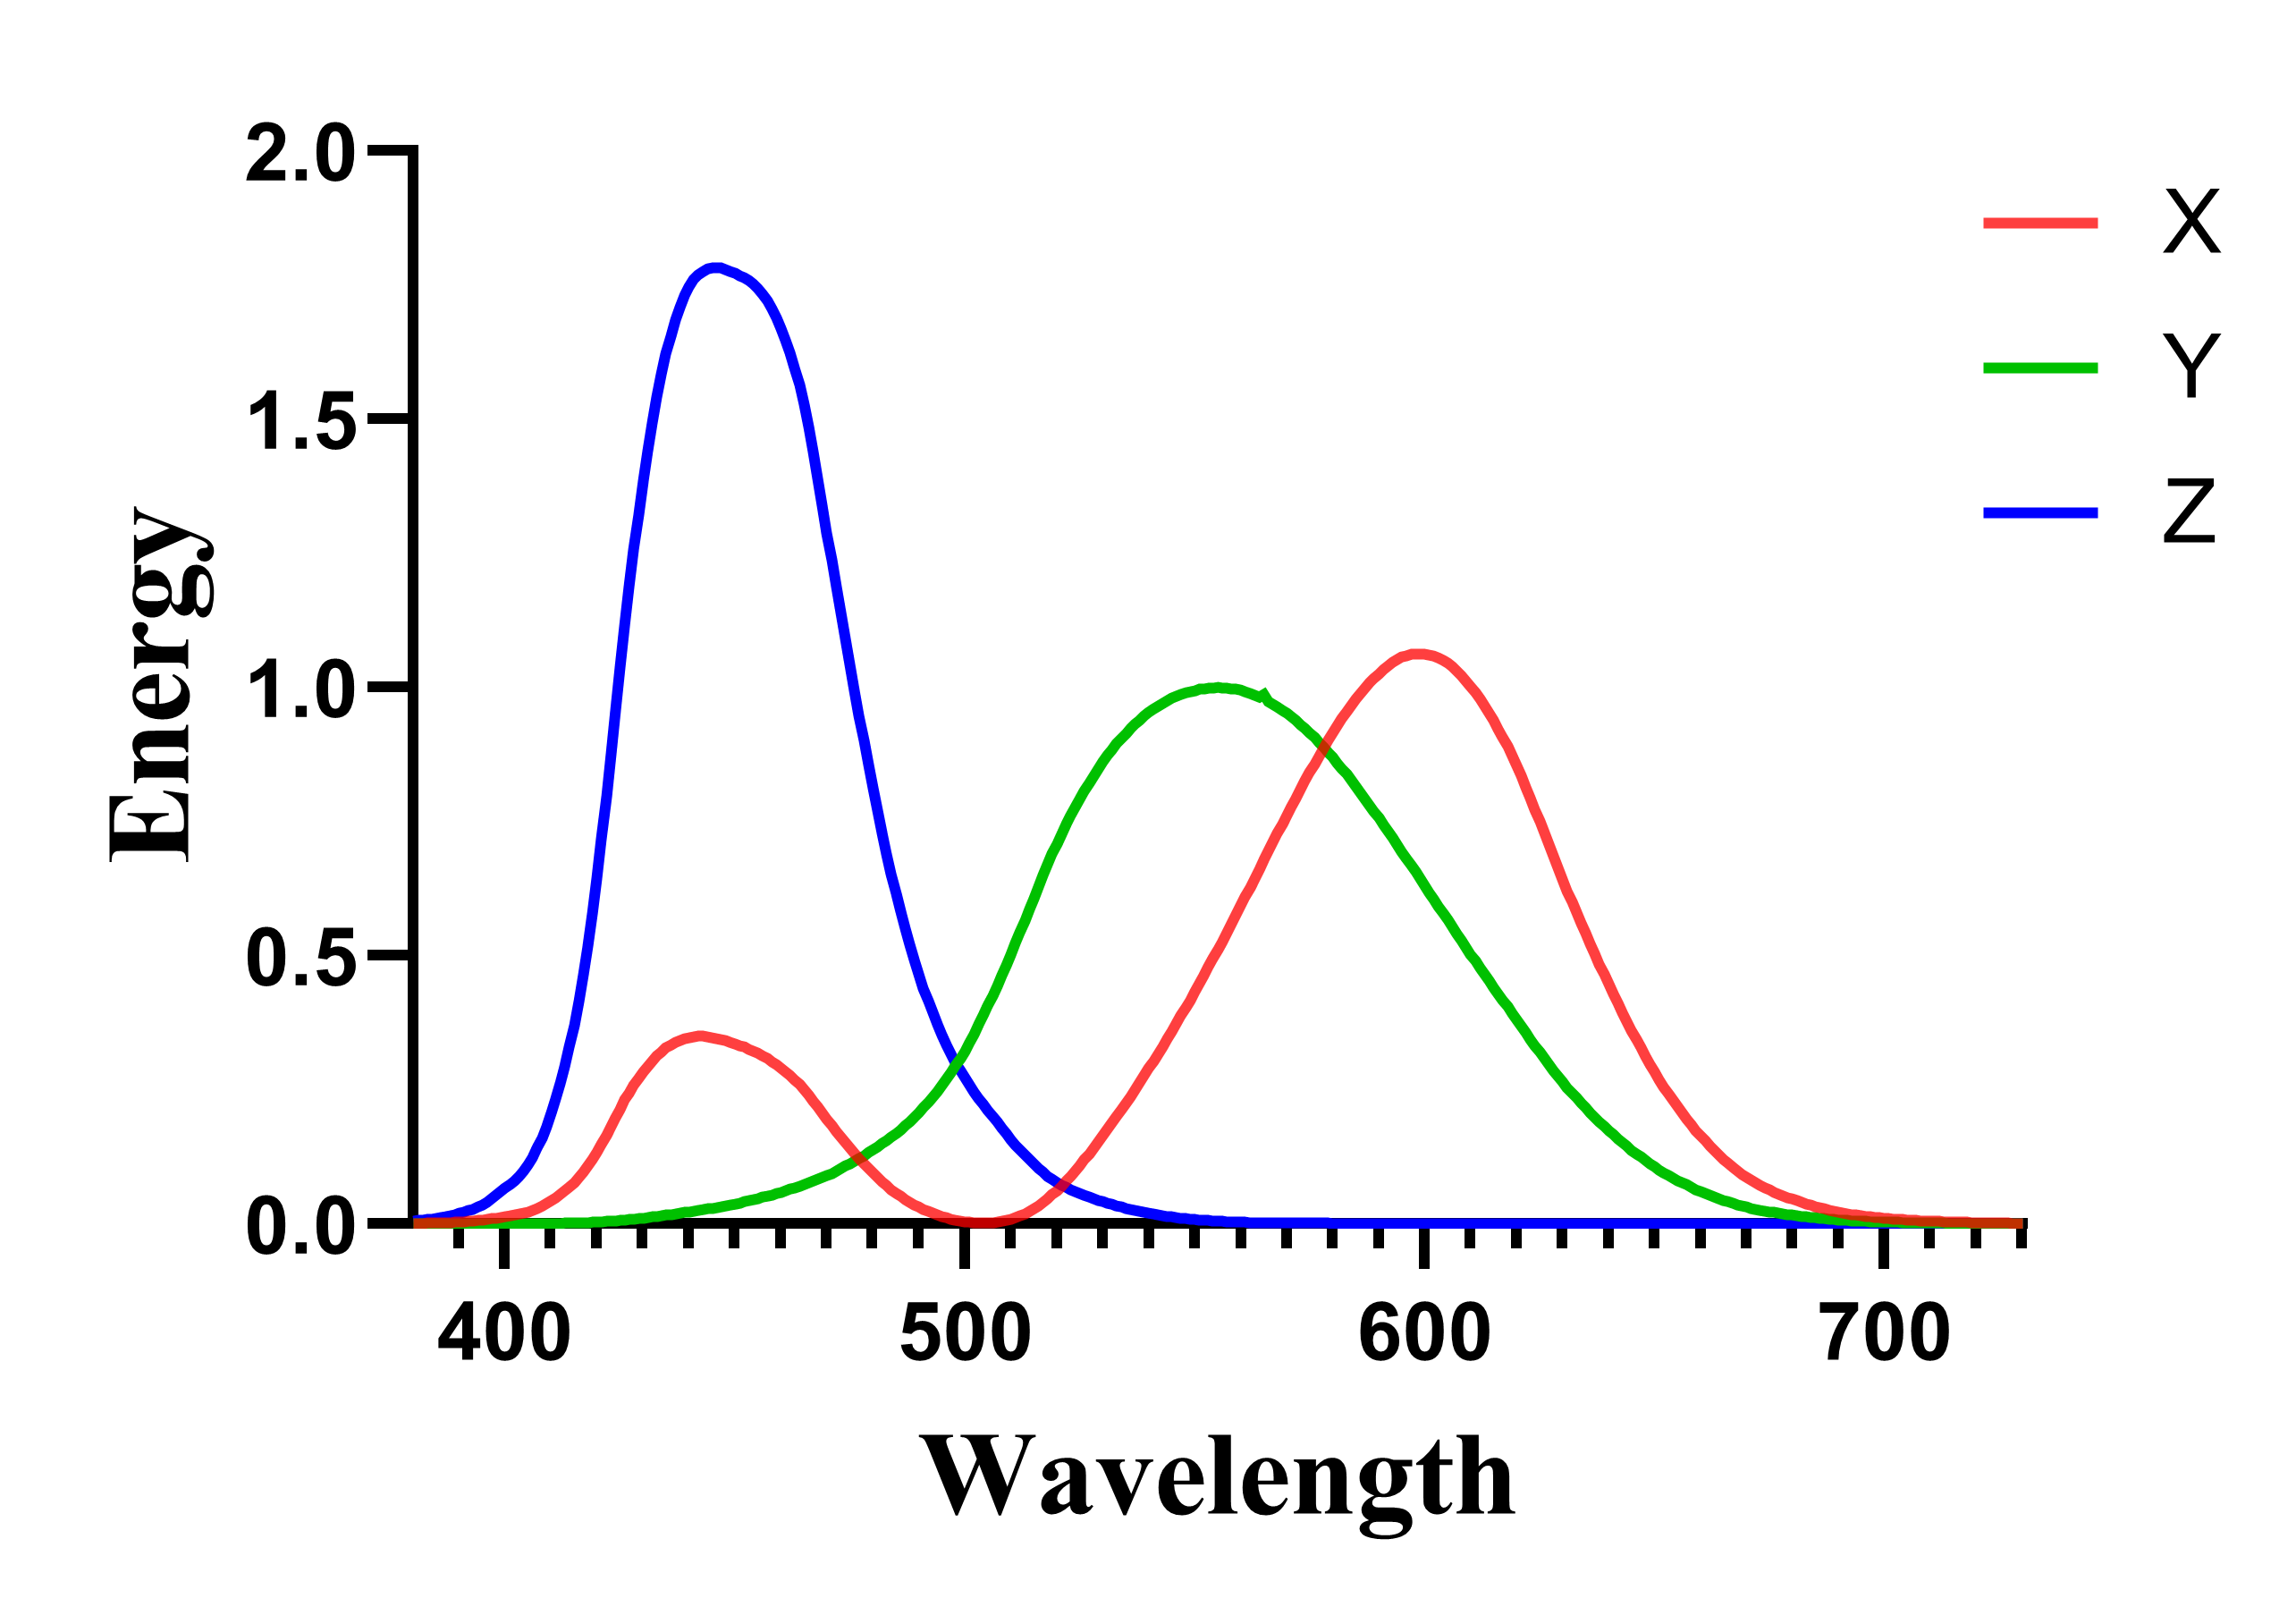
\includegraphics[width=0.5\linewidth]{Styles/figures/en-wa.png}
\caption{CIE 1931 Standard Chroma Observer Spectral tristimulus Values.} 
\end{figure}

\textbf{Step 4: Sample selection by composite metric.}
\subsubsection{Metrics Optimized by Introducing Category Information}
In this section, we will elaborate on how to reasonably adjust the filtering strategy by leveraging the size of the poisoning region in triggers, thereby selecting data that significantly increases the attack success rate. Compared to filtering from the perspective of stealthiness, a filtering strategy aimed at enhancing attack effectiveness requires a pre-training process.
The core technique for sample selection is how to devise advanced metrics (i.e.,
Loss Value, Gradient Norm, and Forgetting Event) to evaluate the importance of samples for poisoning. Our methods are based on the observation and analysis of the drawbacks of current metrics. 
\paragraph{Loss Value}
Given a benign model \(f_{\theta}\) (trained on the benign training set \(D_{tr}\)), the loss value of model on sample \((x_i,y_i)\) can be represented as \(L(f_{\theta}(x_i), y_i)\). We choose samples with the greatest \(\alpha*|D_{tr}|\) values in the subset \(D_t\) are chosen for
poisoning:
\begin{equation}
D_s = arg \max_{D_s\subset D_t}\sum_{(x_i,y_i) \in D_s}L(f_{\theta}(x_i),y_i).
\end{equation}
\paragraph{Gradient Norm}
Given a benign model \(f_{\theta}\) (trained on the benign training set \(D_{tr}\)), the \(l_2-\) gradient norm of model on sample \((x_i,y_i)\) can be represented as \(||\nabla_{\theta} L(f_{\theta}(x_i), y_i)||_2\). We choose samples with the greatest \(\alpha*|D_{tr}|\) values in the subset \(D_t\) are chosen for
poisoning:
\begin{equation}
D_s = arg \max_{D_s\subset D_t}\sum_{(x_i,y_i) \in D_s}||\nabla_{\theta} L(f_{\theta}(x_i), y_i)||_2.
\end{equation}

\paragraph{Forgetting Event} We name the event when a sample \(x_i\) was classified correctly in the previous epoch but incorrectly in the current epoch as a forgetting event of sample \(x_i\). The number of forgetting events happened on sample \(x_i\) during the training process is denoted as \(Num_{forget}(x_i)\). Those samples with the greatest \(\alpha*|D_{tr}|\) forgetting statistics in the subset \(D_t\) are chosen for trigger injection:
\begin{equation}
D_s = arg \max_{D_s\subset D_t}\sum_{(x_i,y_i) \in D_s}Num_{forget}(x_i).
\end{equation}

\paragraph{Remark}
The ultimate goal of proposing these selection criteria is to enhance the effectiveness of clean-label attacks. However, the actual definitions of these criteria do not establish a close connection with the clean-label setting. Additionally, \textbf{\textit{these criteria are trigger-agnostic and fail to propose a simple but effective strategy to optimize the criteria based on the characteristics of the trigger.}} For example, the forgetting event criterion only selects data with high learning difficulty from dataset \(D_{tr}\), and its essence is unrelated to whether the attack is clean-label or dirty-label. What is more, samples are selected independently in the traditional selection strategy. For example, given a subset \(D_{\tilde{s}}\) has been selected for poisoning, the selection of samples \(D_s\backslash D_{\tilde{s}}\) will not be influenced by the already selected samples \(D_{\tilde{s}}\). However, \textit{\textbf{a more effective approach is to seek an overall optimal set rather than a simple combination of individually optimal ones.}}

\paragraph{Our metric}
In the clean-label setting, we believe that data that frequently misclassifies to more classes are more valuable than data that frequently misclassifies to specific classes. Data that frequently misclassifies to more classes can, to some extent, represent data from different classes in a dirty-label scenario, thus bridging the gap between clean-label and dirty-label attacks. It is worth noting that we do not limit the value only to the categories to which the data shifts when a forgetting event occurs. Specifically, we record the distribution of all the categories \(y_e\;(y_e \neq y_i)\) when the sample \((x_i,y_i)\) is misclassified during the pre-training process. \(N_e(y_m,(x_i,y_i))\) represents the number of times sample \((x_i,y_i)\) is misclassified as \(y_m\;(y_m\in Y\;and\;y_m\neq y_i )\). Our principle for designing metrics consists of several parts and thus our design of sample selection strategy can be regarded as a multi-level optimization problem.

\textbf{Principle 1: Select hard samples.} The first design principle aligns with the current mainstream selection principle, which is to identify and poison data that is more difficult to train. Unlike forgetting events, we relax some constraints. We believe that sample that is frequently misclassified is just as difficult to learn as data that often experiences forgetting events. The number of misclassification events (e.g., events that be misclassified as \(y_m\;(y_m \neq y_i)\)) that happened on sample \((x_i,y_i)\) during the training process is denoted as \(Num_{e}(x_i)\) (\(N{e}((x_i,y_i),y_m)\)). Those samples with the greatest \(\alpha*|D_{tr}|\) misclassification statistics in the subset \(D_t\) should enjoy prior selection for trigger injection:
\begin{equation}
D_s = arg \max_{D_s\subset D_t}\sum_{(x_i,y_i) \in D_s}N{e}((x_i,y_i),y_m).
\end{equation}

\textbf{Principle 2: Ensure category diversity.} The second design principle is to select samples \(D_s\) that cover more classes of the training set \(D_{tr}\) as much as possible. Consequently, the selected set \(D_s\) exhibits higher similarity and more robust coupling with the features of non-target classes, thereby rendering it challenging for the model to accurately classify \(D_s\) as the intended target class \(y_t\). Therefore, the model is more likely to learn the strong correspondence between the features of the injected trigger and the target label \(y_t\) to enhance the effectiveness of the backdoor attack. We use \(Exists(N_e((x_i,y_i),y_m))\) to represent whether there is a misclassification event that the model misclassify the \(x_i\) as \(y_m\;(y_m \neq y_i)\)) during the training process when function \(Exists(N_e((x_i,y_i),y_m))\) output \(1\) and \(0\) otherwise. Those samples with the greatest \(\alpha*|D_{tr}|\)  statistics in the subset \(D_t\) should enjoy prior selection for trigger injection:
\begin{equation}
D_s = arg \max_{D_s\subset D_t}\sum_{(x_i,y_i) \in D_s}Exists(N_e((x_i,y_i),y_m)).
\end{equation}

\textbf{Principle 3: Ensure the balance in category proportions.} The last design principle is to ensure that each category occupies a significant proportion in the filtered samples \(D_s\). In the training dataset, there exist variations in the degree of similarity among diverse categories. For instance, the resemblance among animal classifications exceeds that among plant categories. Consequently, when a particular animal serves as the target label \(y_t\), the volume of data erroneously labeled as plants during the pre-training phase will decline notably in comparison to data misidentified as other animals. According to the \textbf{Principle 1}, the image set that resembles the samples whose labels have low similarity with the target label will be difficult to select, thus weakening the consideration in \textbf{Principle 2}. The specific set that the model misclassifies as labels with minimal similarity to the intended target label \(y_t\) poses a greater challenge for the model to accurately classify within the target category. This difficulty makes it easier for the model to establish a strong connection between the backdoor trigger features and the target label \(y_t\), thereby increasing the effectiveness of the attack. We use \(\mu\) to represent the mean of \(\{N{e}((x_i,y_i),y_m)(y_m\neq y_t)\}\). The subset \(D_t\) including \(\alpha*|D_{tr}|\) is expected to cover all categories in relatively balanced proportions:
\begin{equation}
D_s = arg \min_{D_s\subset D_t}\sum_{(x_i,y_i) \in D_s}||N_{e}((x_i,y_i),y_m)-\mu||_2.
\end{equation}

\paragraph{Implementation}
The aforementioned principles exhibit a degree of conflict with each other. Determining the appropriate magnitude of adjustment for the decision-making weights of these principles is of paramount importance. Our extensive experimental analysis has revealed that the allocation of these weights is contingent upon the coupling degree between trigger feature learning and non-target class features. In this paper, we propose a simple yet effective guidance method. Triggers with larger poisoning areas rely more on Principle 2 and Principle 3 than those triggers with smaller backdoor areas. We devise distinct negative functions \(N_F\) to facilitate the reduction of weights at varied rates (e.g.,\(O(\log(n)), O(n), O(n^2)), \;and\;O(e^n)\)) based on their relative proportions \(n=\frac{N{e}((x_i,y_i),y_m)}{\sum_{y_j \neq y_t} N{e}((x_i,y_i),y_j)}(y_m \neq y_t)\). A strategy with a gradual weight reduction emphasizes \textbf{Principle 1}, whereas a rapid reduction favors \textbf{Principle 2} and \textbf{Principle 3}. What is more, we also propose a strategy, dubbed forget, to only consider \textbf{Principle 1}, and a strategy, dubbed num, to only consider \textbf{Principle 2}. Details are presented in Algorithm 2-5.
\begin{breakablealgorithm}
\caption{Metric Calculation with Negative Function $N_F$ at $O(\log(n))$}
\renewcommand{\algorithmicrequire}{\textbf{Input : }}
\begin{algorithmic}[0]
\algorithmicrequire Train Dataset $D_{tr}$, Target Label $y_t$, Misclassification Events $N_{e}((x_i,y_i),y_m)$\\
\textbf{Output : } Calculated Metric of Samples \\
\FOR{image $(x_i,y_t) \in D_{tr}$}
\STATE $Num[y_m] = 0$\\
    \FOR{$y_m \in Y$}
        \STATE $Num[y_m] = Num[y_m] + N_{e}((x_i,y_t),y_m)$\\
    \ENDFOR
\ENDFOR
\FOR{$y_m \in Y$}
    \STATE $Sum = Sum + log(1+Num[y_m])$\\
\ENDFOR
\FOR{$y_m \in Y$}
    \STATE $Cls[y_m] = 1 - \frac{log(1+Num[y_m])}{Sum}$\\
\ENDFOR
\FOR{image $(x_i,y_t) \in D_{tr}$}
\STATE $Metric[x_i] = 0$\\
    \FOR{$y_m \in Y$}
        \STATE $Metric[x_i] = Metric[x_i] + Cls[y_m]*N_{e}((x_i,y_t),y_m)$
    \ENDFOR
\ENDFOR
\end{algorithmic}
\end{breakablealgorithm}

\section{Experiments}
\subsection{Main settings}
\paragraph{Dataset and Model.}
 To clearly demonstrate the impact of category count on trigger feature learning across different poisoning regions, we conduct a series of systematic modifications to the CIFAR-100 dataset. Specifically, we meticulously select subsets with varying numbers of categories from CIFAR-100 for our experiments, terming these subsets CIFARX-N \((N\in\{10,20,\dots,100\})\).
\paragraph{Baseline Selection.}
 Compared to the aforementioned visible attacks, we also introduce BppAttack as a benchmark characterized by enhanced visual covertness but increased training complexity. BppAttack utilizes image quantization as the trigger feature and requires a higher poisoning rate, adversarial training, and label flipping to maintain effective attack performance. BppAttack employs image quantization as its trigger feature and necessitates a higher poisoning rate, adversarial training, and label flipping to sustain effective attack efficacy. Its primary advantage is its ability to maintain stealthiness by incorporating smoother and more difficult-to-detect perturbations without the need for training a trigger generator.

\paragraph{Attack Setup on CIFARX.}
For BadNets, a \(3 × 3\) checkerboard pattern is utilized as the trigger. For the Blended attack, a Hello-Kitty image is selected as the trigger and blended with the original images, with a transparency parameter of \(0.2\). Across all these attacks, \(10\%\) of the samples from the target class (representing \(1\%\) of the total samples) are poisoned, with the first class ("airplane") designated as the target class.

\subsection{Superiority of MultiBpp Attack}

\subsubsection{Attack Setup.}
To objectively describe the superiority of MultiBpp, we adopt the same experimental setup as BppAttack (\citet{wang2022bppattack}). Specifically, the default bit depth of BppAttack in the original work is \(5\), which can be seen as \(32:32:32\) in quantization. We use Base to represent the attack by quantizing the images with \(32:32:32\) without any other process. Furthermore, we introduce the clean-label variants of Blend (dubbed 'Blend-C') to elaborate on the efficiency of the MultiBpp attack. For the Blended attack, a Hello-Kitty image is selected as the trigger and blended with the original images, with a transparency parameter of \(0.2\). Drawing upon the two strategies outlined in Section 3.2.1 for selecting poisoning data based on stealthiness, we devise two corresponding MultiBpp triggers. One involves poisoning exclusively the blue channel, which exhibits lower sensitivity to human perception, whereas the other implements differential poisoning across all channels. The quantization setting of poisoning intensity in RGB channels is approximately designed as \(3:6:1\) according to the contribution to the brightness of images. (todo. poisoned images)

The first class ("airplane") is designated as the target class. The BppAttack gets a poor attack success rate \((12.5\%)\) with \(2.5\%\) samples poisoned upon CIFAR10 (\cite{krizhevsky2009learning}) using Resnet18 (\cite{he2016deep}) and \(2.5\%\) is selected as the poisoning rate to construct all attacks. We assess all backdoor attacks using two classification metrics: CleanACC and ASR, which are denoted at \textbf{Section 3.1.2}. CleanACC (dubbed 'BA') represents the average prediction accuracy of all clean testing samples over \(20\) epochs, whereas ASR represents the average accuracy of their poisoned counterparts over \(20\) epochs. The objective of adversaries is to ensure attack effectiveness, characterized by a high ASR, while preserving the model's standard functionality, indicated by a high BA. 

\subsubsection{Result Analysis.}
\begin{figure*}[h]
\setlength{\itemsep}{-10pt}
\centering
\subfigure[\fontsize{10}{12}\selectfont Benign]{
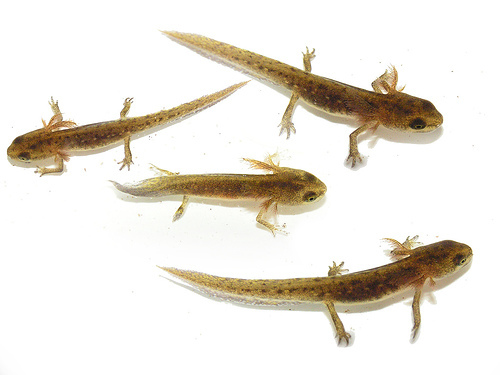
\includegraphics[width=0.2\linewidth]{Styles/figures/2_Benign.JPEG}}
\subfigure[\fontsize{10}{12}\selectfont Base]{
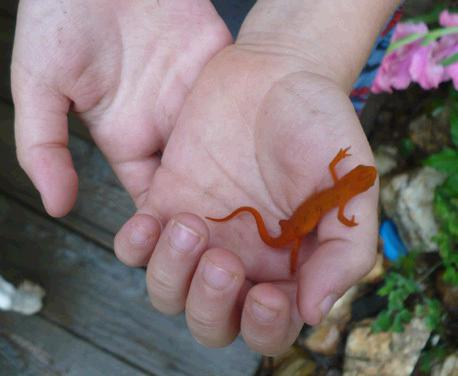
\includegraphics[width=0.2\linewidth]{Styles/figures/Base.jpeg}}
\subfigure[\fontsize{10}{12}\selectfont BppAttack]{
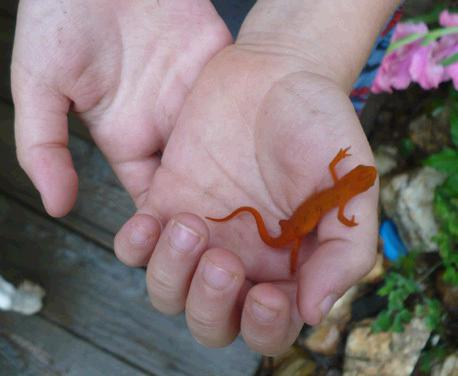
\includegraphics[width=0.2\linewidth]{Styles/figures/BppAttack.jpeg}}
\subfigure[\fontsize{10}{12}\selectfont Blend-C]{
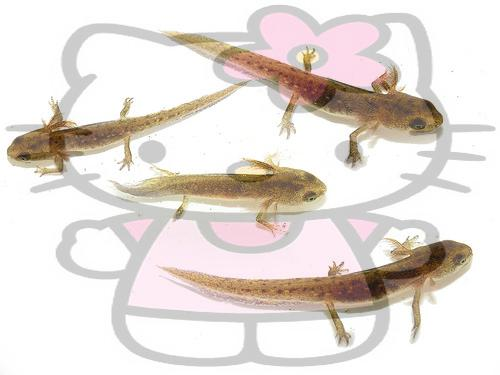
\includegraphics[width=0.2\linewidth]{Styles/figures/2_blended_image_0.2.jpeg}}
\subfigure[\fontsize{10}{12}\selectfont 255:255:8]{
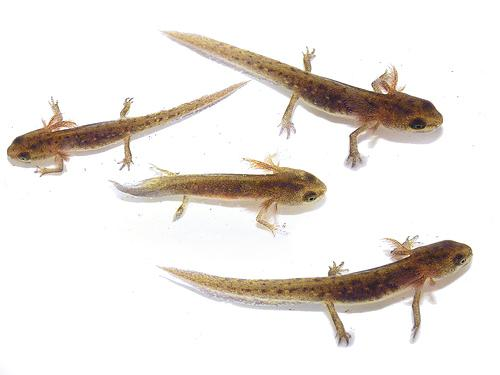
\includegraphics[width=0.2\linewidth]{Styles/figures/2_Q255_255_8.jpeg}}
\subfigure[\fontsize{10}{12}\selectfont 255:255:12]{
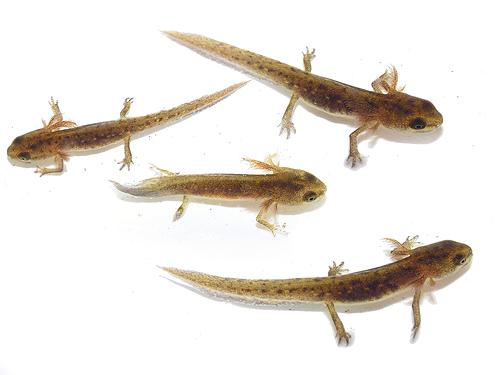
\includegraphics[width=0.2\linewidth]{Styles/figures/2_Q255_255_12.jpeg}}
\subfigure[\fontsize{10}{12}\selectfont 24:48:8]{
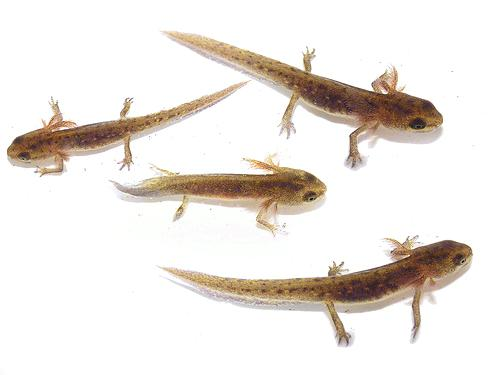
\includegraphics[width=0.2\linewidth]{Styles/figures/2_Q24_48_8.jpeg}}
\subfigure[\fontsize{10}{12}\selectfont 36:72:12]{
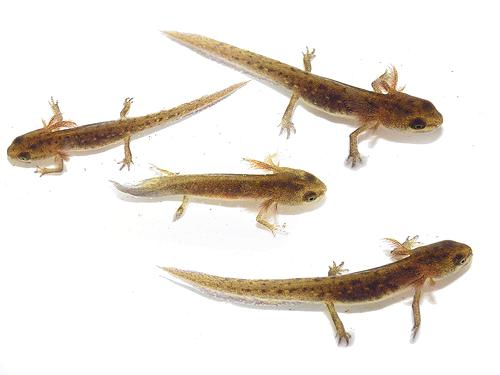
\includegraphics[width=0.2\linewidth]{Styles/figures/2_Q36_72_12.jpeg}}
\subfigure[\fontsize{10}{12}\selectfont 8:255:255]{
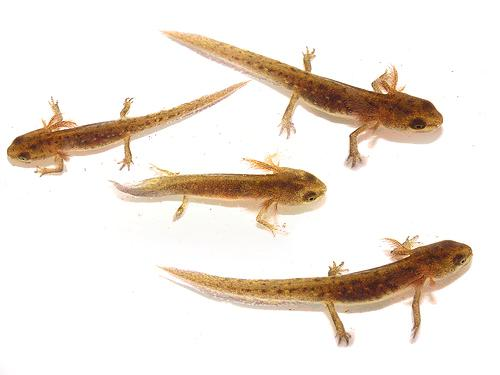
\includegraphics[width=0.2\linewidth]{Styles/figures/2_Q8_255_255.jpeg}}
\subfigure[\fontsize{10}{12}\selectfont 255:8:255]{
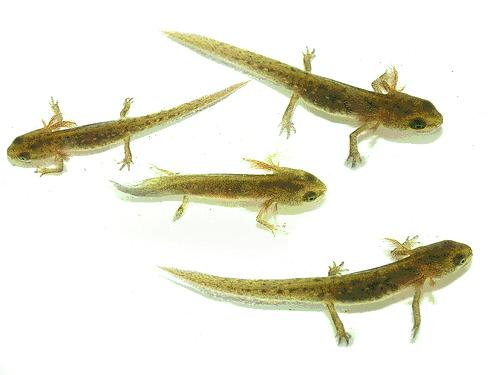
\includegraphics[width=0.2\linewidth]{Styles/figures/2_Q255_8_255.jpeg}}
\subfigure[\fontsize{10}{12}\selectfont 12:255:255]{
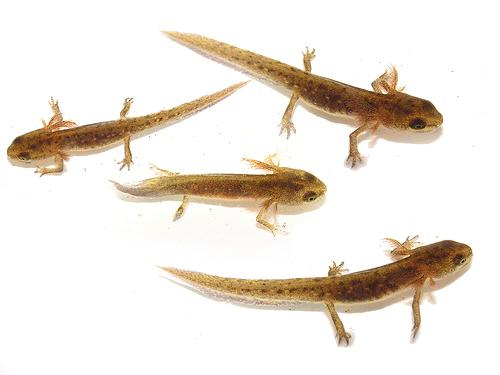
\includegraphics[width=0.2\linewidth]{Styles/figures/2_Q12_255_255.jpeg}}
\subfigure[\fontsize{10}{12}\selectfont 255:12:255]{
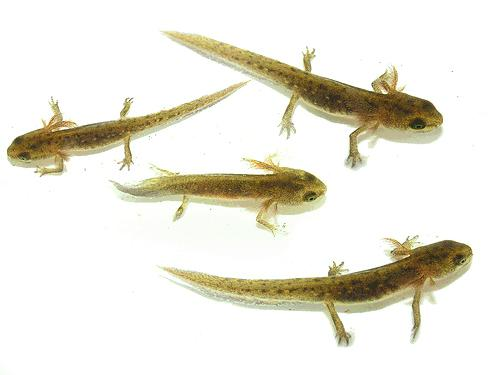
\includegraphics[width=0.2\linewidth]{Styles/figures/2_Q255_12_255.jpeg}}
\caption{Images poisoned by different attacks. The images in the CIFAR-10 dataset have relatively low pixel quality, making it difficult to compare the subtle differences in visibility among different methods. Therefore, we have selected images from the training set of the same category in the ImageNet dataset, which has higher quality, as demonstrations. Methods a-d involve randomly selecting poisoned data, while methods e-l involve selecting images that are more concealed after poisoning.} 
\end{figure*}
\paragraph{Stealthiness}
The original BppAttack randomly selects data for poisoning. To maintain the stealthiness of the trigger, BppAttack needs to adopt a smaller quantization step \((32:32:32)\), which makes it difficult for the trigger features to be learned. Our method further optimizes based on two observations: 1. Images e, i, and j at Figure 2 correspond to the effects of poisoning the blue, red, and green channels, respectively. From a comparison of human visibility, it can be seen that the human eye is much less sensitive to the blue channel than to the other channels. Therefore, increasing the poisoning intensity in the blue channel can still maintain invisibility to the human eye. 2. According to Figure 2, images a and b show that within the same category of the same dataset, there are images with vastly different sensitivities to trigger features from a visibility perspective. By reasonably selecting data, the stealthiness of the trigger can be well ensured. The comparison between images d and b indicates that data that is insensitive to MultiBpp in terms of human visibility is more sensitive to Blend attacks. Moreover, performing a Blend attack based on image b will provide better concealment compared to attack based on image d. Therefore, The strategy for selecting insensitive data from the perspective of stealthiness still needs to consider the trigger features. 

\begin{table*}[h]
\resizebox{.98\columnwidth}{!}{
\centering
\begin{tabular}{|c|c|c|c|c|c|c|c|}
\hline
\multicolumn{3}{|c|}{\textit{Attack}} & \multicolumn{2}{|c|}{\textit{Metric}}&\multicolumn{3}{c|}{\textit{Attack Setting}}\\
\cline{1-8}

\multirow{1}{*}{Type} & no. & Method & BA(avg) & ASR(avg) & Clean-label & Training Control & Stealthy\\
\hline

\multirow{4}{*}{Benchmark} & a & Benign & - & \textbf{95.0\%} & \faCheckCircle & \faTimesCircle & \faCheckCircle \\
%\cline{2-8}

\multirow{4}{*}{} & b & Base & \textbf{\textcolor{red}{8.2\%}} & 94.8\% & \faCheckCircle & \faTimesCircle & \faCheckCircle \\
%\cline{2-8}

\multirow{4}{*}{} & c & BppAttack & \textbf{\textcolor{red}{12.5\%}} & 94.5\% & \textcolor{red}{\faTimesCircle} & \textcolor{red}{\faCheckCircle} & \faCheckCircle \\
%\cline{2-8}

\multirow{4}{*}{} & d & Blend-C & \textbf{66.4\%} & 94.3\% & \faCheckCircle & \faTimesCircle & \textcolor{red}{\faTimesCircle} \\
\cline{1-8}

\multirow{4}{*}{MultiBpp} & e & 255:255:8 & 68.6\% & 94.8\% & \faCheckCircle & \faTimesCircle & \faCheckCircle \\
%\cline{2-8}

\multirow{4}{*}{} & f & 255:255:12 & 60.0\% & \textbf{94.9\%} & \faCheckCircle & \faTimesCircle & \faCheckCircle \\
%\cline{2-8}

\multirow{4}{*}{} & g & 24:48:8 & \textbf{76.6\%} & 94.7\% & \faCheckCircle & \faTimesCircle & \faCheckCircle \\
%\cline{2-8}

\multirow{4}{*}{} & h & 36:72:12 & 57.7\% & 94.6\% & \faCheckCircle & \faTimesCircle & \faCheckCircle \\
\cline{1-8}

\multirow{1}{*}{} & i & 8:255:255 & \textbf{84.1\%} & \textbf{94.7\%} & \faCheckCircle & \faTimesCircle & \textcolor{red}{\faTimesCircle} \\
%\cline{2-8}

\multirow{1}{*}{MultiBpp} & j & 255:8:255 & 72.2\% & 94.3\% & \faCheckCircle & \faTimesCircle & \textcolor{red}{\faTimesCircle} \\
%\cline{2-8}

\multirow{1}{*}{(others)} & k & 12:255:255 & 67.6\% & 94.5\% & \faCheckCircle & \faTimesCircle & \textcolor{red}{\faTimesCircle} \\
%\cline{2-8}

\multirow{1}{*}{} & l & 255:12:255 & 73.8\% & 94.5\% & \faCheckCircle & \faTimesCircle & \textcolor{red}{\faTimesCircle} \\
\cline{2-8}
\hline
\end{tabular}
}
\caption{Performance of attacks by poisoning 2.5\% samples of CIFAR10. \textbf{\textcolor{red}{Red}} represents the negative performance and requirement of attacks. \(N_p^R:N_p^G:N_p^B\) in \textbf{Method} of MultiBpp represents the concrete quantization setting of poisoning intensity in RGB channels. Furthermore, Bengin serves as the original training period without being poisoned by backdoor attacks.}
\end{table*}

\paragraph{Attack Performance}
According to Tables 1c and 1b, even under strong conditions such as label flipping and controlled training, BppAttack still cannot guarantee the effectiveness of the attack (ASR of 12.5\%) at a poisoning rate of 2.5\%. As shown in Tables e-h, our proposed method significantly improves the attack effect under the clean-label setting and with only the dataset being poisoned. Specifically, MultiBpp achieves an ASR of 76.6\% with a quantization step of 24:48:8 while maintaining a higher BA. Furthermore, Tables 1i-l indicate that there are still differences in efficiency when poisoning different channels. Specifically, poisoning the red and green channels yields better results. We speculate that the model also infers during the learning process that features in the red and green channels are more valuable, leading to different learning sensitivities. Tables 1e and f, as well as g and h, both indicate that increasing the quantization step generally improves the attack success rate. It is worth noting that a comparison between f and h suggests that there are exceptions to this rule. We speculate that the learning effectiveness of poisoning features is not solely influenced by the intensity of quantization efforts. Specifically, in scenarios with lower quantization intensity (f and h), the model needs to focus on features from three channels when learning h, whereas it only needs to attend to features from one channel when learning f. In such scenarios, the model finds it easier to learn f rather than h, which involves a greater quantization effort.
\subsection{Superity of Trigger-specific Selection(todo name)}
\subsubsection{Attack Setup.}
We conduct experiments on two benchmark datasets, including CIFAR-10 and CIFAR-100 (\cite{krizhevsky2009learning}), with ResNet-18 (\cite{he2016deep}). We compare our plug-in methods against the standard version with random selection (dubbed 'vanilla') and existing sample selection strategies based on various metrics (such as forgetting events, gradient norm, and loss value). To objectively describe the superiority of our method, we adopt the same experimental setup as the setting devised by \citet{gao2023not}. We introduce the clean-label variants of two classic poisoned-label attacks: BadNets (dubbed 'BadNets-C') as a representative of attacks with small poisoning area, and an attack utilizing a blended strategy (dubbed 'Blended-C') as a representative of attacks poisoning the whole image, by poisoning samples only from the target class. For BadNets, a \(3 \times 3\) checkerboard pattern is utilized as the trigger. For the Blended attack, a Hello-Kitty image is selected as the trigger and blended with the original images, with a transparency parameter of \(0.2\). Considering that the main objective of this chapter is to demonstrate the superiority of the filtering strategy in enhancing attack effectiveness, the selection of poisoned data for the MultiBpp attack in this chapter will be entirely consistent with that of other attacks. The stealthiness of the trigger is ensured by the quantization strength. In CIFAR10, we adopt the more stealthy settings of 255:255:12 and 36:72:12 from Section 4.2 as the attack configurations. Across all these attacks upon CIFAR10, \(10\%\) of the samples from the target class (representing \(1\%\) of the total samples) are poisoned, with the first class ("airplane") designated as the target class. We use the same evaluation metric mentioned in Section 4.2.1.
\paragraph{Attack Setup on CIFAR-100.(todo)}
For BadNets, a \(3 × 3\) checkerboard pattern is utilized as the trigger. For the Blended attack, a Hello-Kitty image is selected as the trigger and blended with the original images, with a transparency parameter of \(0.2\). Across all these attacks, \(10\%\) of the samples from the target class (representing \(1\%\) of the total samples) are poisoned, with the first class ("airplane") designated as the target class.
\subsubsection{Result Analysis.}
\begin{table*}[h]
\resizebox{.98\columnwidth}{!}{
\centering
\begin{tabular}{|c|c|c|c|c|c|c|c|}
\hline
\multicolumn{3}{|c|}{\textit{Method}} & \multicolumn{}{|c|}{\textit{Metric}}&\multicolumn{4}{c|}{\textit{Attack}}\\
\cline{1-8}

\multirow{1}{*}{Type} & no. & Selection &  & Badnets-C & Blended-C & 255:255:12 & 36:72:12\\
\hline

\multirow{8}{*}{Benchmark} & \multirow{2}{*}{a} & \multirow{2}{*}{Vanilla} & BA & 94.42\% & 94.90\% & 94.51\% & 94.95\% \\
%\cline{4-8}

\multirow{8}{*}{} & \multirow{2}{*}{} & \multirow{2}{*}{} & ASR & 37.24\% & 53.41\% & \textcolor{red}{1.37\%} & \textcolor{red}{1.16\%} \\
%\cline{2-8}
\multirow{8}{*}{} & \multirow{2}{*}{b} & \multirow{2}{*}{Loss Value} & BA & 94.71\% & \textbf{95.10\%} & 94.84\% & 94.76\% \\
%\cline{4-8}
\multirow{8}{*}{} & \multirow{2}{*}{} & \multirow{2}{*}{} & ASR & 52.71\% & 59.43\% & 28.02\% & 47.85\% \\
%\cline{2-8}
\multirow{8}{*}{} & \multirow{2}{*}{c} & \multirow{2}{*}{Gradient Norm} & BA & 94.45\% & 94.77\% & \textbf{95.04\%} & \textbf{95.03\%} \\
%\cline{4-8}
\multirow{8}{*}{} & \multirow{2}{*}{} & \multirow{2}{*}{} & ASR & 52.56\% & 58.45\% & 38.26\% & 53.28\% \\
%\cline{2-8}
\multirow{8}{*}{} & \multirow{2}{*}{d} & \multirow{2}{*}{Forgetting Event} & BA & \textbf{94.90\%} & 94.55\% & 94.92\% & 94.90\% \\
%\cline{4-8}
\multirow{8}{*}{} & \multirow{2}{*}{} & \multirow{2}{*}{} & ASR & \textbf{71.74\%} & \textbf{71.05\%} & \textbf{74.39\%} & \textbf{78.10\%} \\
\cline{1-8}
\multirow{8}{*}{Our Method} & \multirow{2}{*}{e} & \multirow{2}{*}{Res-log} & BA & \textbf{94.98\%} & 94.73\% & 94.54\% & 94.82\% \\
%\cline{4-8}
\multirow{8}{*}{} & \multirow{2}{*}{} & \multirow{2}{*}{} & ASR & \textbf{82.13\%} & 82.34\% & 77.10\% & 80.20\% \\
%\cline{2-8}
\multirow{8}{*}{} & \multirow{2}{*}{f} & \multirow{2}{*}{Res-linear} & BA & 94.71\% & 94.31\% & 94.21\% & 94.63\% \\
%\cline{4-8}
\multirow{8}{*}{} & \multirow{2}{*}{} & \multirow{2}{*}{} & ASR & 68.65\% & 82.31\% & 76.73\% & 83.07\% \\
%\cline{2-8}
\multirow{8}{*}{} & \multirow{2}{*}{g} & \multirow{2}{*}{Res-square} & BA & 94.94\% & 94.38\% & 94.58\% & 94.59\% \\
%\cline{4-8}
\multirow{8}{*}{} & \multirow{2}{*}{} & \multirow{2}{*}{} & ASR & 78.76\% & \textbf{84.88\%} & \textbf{82.54\%} & \textbf{83.88\%} \\
%\cline{2-8}
\multirow{8}{*}{} & \multirow{2}{*}{h} & \multirow{2}{*}{Res-exp} & BA & 94.47\% & \textbf{94.80\%} & \textbf{94.72\%} & \textbf{94.85\%} \\
%\cline{4-8}
\multirow{8}{*}{} & \multirow{2}{*}{} & \multirow{2}{*}{} & ASR & 76.50\% & 71.81\% & 53.92\% & 62.28\% \\
\cline{2-8}
\hline
\end{tabular}
}
\caption{Performance of attacks by poisoning 1\% samples of CIFAR10. \textbf{\textcolor{red}{Red}} represents the negative performance of attacks. \(N_p^R:N_p^G:N_p^B\) in \textbf{Method} of MultiBpp represents the concrete quantization setting of poisoning intensity in RGB channels.}
\end{table*}
\paragraph{Analysis on CIFAR10}
From the comparison between images {e, f, g} and {b, c, d}, it can be concluded that incorporating considerations of category diversity in data filtering can significantly enhance attack effectiveness. Specifically, for BadNets attacks, our method, res-log, outperforms the currently best-performing forgetting event metric by \(11\) percentage points in Attack Success Rate (ASR), corresponding to \(71.74\%\) and \(82.13\%\), respectively. For Blend attacks, our method exceeds the forgetting event metric by approximately \(14\) percentage points in ASR, corresponding to \(71.05\%\) and \(84.88\%\), respectively. Regarding the newly proposed multi-bpp method in this paper, there is also an ASR improvement of over \(6\) percentage points. 

The selection criteria for e-h are designed to incorporate considerations of category diversity from a light to a heavy degree. From the comparison between d and h across various attacks, it can be seen that excessively emphasizing category diversity is not the optimal strategy. Particularly for attack methods where the poisoning region covers the entire image (Blended-C, MultiBpp), the consideration of category diversity has a greater impact on the filtering strategy. The attack can achieve the optimal combination of poisoned data under the more aggressive strategy g. However, excessively emphasizing category diversity can also lead to a greater decrease in Attack Success Rate (ASR). It is worth noting that BadNets attacks belong to the type of attacks that poison specific regions of images. Therefore, the learning of trigger features relies more on whether the samples themselves are difficult to learn, and thus considerations of category diversity should be introduced to a lesser extent. The attack can achieve the optimal combination of poisoned data under the less aggressive strategy e. Therefore, the choice of data filtering strategy needs to take into account the characteristics of the trigger itself. By reasonably designing a filtering strategy that incorporates considerations of category diversity based on the trigger characteristics, an optimal set of poisoned data can be obtained.
\begin{table*}[h]
\resizebox{.98\columnwidth}{!}{
\centering
\begin{tabular}{|c|c|c|c|c|c|c|c|}
\hline
\multicolumn{3}{|c|}{\textit{Method}} & \multicolumn{}{|c|}{\textit{Metric}}&\multicolumn{2}{c|}{\textit{Poisoning Rate $\alpha=0.1\%$}}&\multicolumn{2}{c|}{\textit{Poisoning Rate $\alpha=0.2\%$}}\\
\cline{1-8}

\multirow{1}{*}{Type} & no. & Selection &  & Badnets-C & Blended-C & Badnets-C & Blended-C\\
\hline

\multirow{8}{*}{Benchmark} & \multirow{2}{*}{a} & \multirow{2}{*}{Vanilla} & BA & 94.42\% & 94.90\% & 94.51\% & 94.95\% \\
%\cline{4-8}

\multirow{8}{*}{} & \multirow{2}{*}{} & \multirow{2}{*}{} & ASR & 37.24\% & 53.41\% & \textcolor{red}{1.37\%} & \textcolor{red}{1.16\%} \\
%\cline{2-8}
\multirow{8}{*}{} & \multirow{2}{*}{b} & \multirow{2}{*}{Loss Value} & BA & 94.71\% & \textbf{95.10\%} & 94.84\% & 94.76\% \\
%\cline{4-8}
\multirow{8}{*}{} & \multirow{2}{*}{} & \multirow{2}{*}{} & ASR & 52.71\% & 59.43\% & 28.02\% & 47.85\% \\
%\cline{2-8}
\multirow{8}{*}{} & \multirow{2}{*}{c} & \multirow{2}{*}{Gradient Norm} & BA & 94.45\% & 94.77\% & \textbf{95.04\%} & \textbf{95.03\%} \\
%\cline{4-8}
\multirow{8}{*}{} & \multirow{2}{*}{} & \multirow{2}{*}{} & ASR & 52.56\% & 58.45\% & 38.26\% & 53.28\% \\
%\cline{2-8}
\multirow{8}{*}{} & \multirow{2}{*}{d} & \multirow{2}{*}{Forgetting Event} & BA & \textbf{94.90\%} & 94.55\% & 94.92\% & 94.90\% \\
%\cline{4-8}
\multirow{8}{*}{} & \multirow{2}{*}{} & \multirow{2}{*}{} & ASR & \textbf{71.74\%} & \textbf{71.05\%} & \textbf{74.39\%} & \textbf{78.10\%} \\
\cline{1-8}
\multirow{8}{*}{Our Method} & \multirow{2}{*}{e} & \multirow{2}{*}{Res-log} & BA & \textbf{94.98\%} & 94.73\% & 94.54\% & 94.82\% \\
%\cline{4-8}
\multirow{8}{*}{} & \multirow{2}{*}{} & \multirow{2}{*}{} & ASR & \textbf{82.13\%} & 82.34\% & 77.10\% & 80.20\% \\
%\cline{2-8}
\multirow{8}{*}{} & \multirow{2}{*}{f} & \multirow{2}{*}{Res-linear} & BA & 94.71\% & 94.31\% & 94.21\% & 94.63\% \\
%\cline{4-8}
\multirow{8}{*}{} & \multirow{2}{*}{} & \multirow{2}{*}{} & ASR & 68.65\% & 82.31\% & 76.73\% & 83.07\% \\
%\cline{2-8}
\multirow{8}{*}{} & \multirow{2}{*}{g} & \multirow{2}{*}{Res-square} & BA & 94.94\% & 94.38\% & 94.58\% & 94.59\% \\
%\cline{4-8}
\multirow{8}{*}{} & \multirow{2}{*}{} & \multirow{2}{*}{} & ASR & 78.76\% & \textbf{84.88\%} & \textbf{82.54\%} & \textbf{83.88\%} \\
%\cline{2-8}
\multirow{8}{*}{} & \multirow{2}{*}{h} & \multirow{2}{*}{Res-exp} & BA & 94.47\% & \textbf{94.80\%} & \textbf{94.72\%} & \textbf{94.85\%} \\
%\cline{4-8}
\multirow{8}{*}{} & \multirow{2}{*}{} & \multirow{2}{*}{} & ASR & 76.50\% & 71.81\% & 53.92\% & 62.28\% \\
\cline{2-8}
\hline
\end{tabular}
}
\caption{Performance of attacks upon CIFAR100.}
\end{table*}
\paragraph{Analysis on CIFAR100}
\subsection{Ablation Study}

\section{Conclusion}
\bibliographystyle{plainnat}  % 使用 natbib 提供的样式
\bibliography{Styles/neurips25} 
\begin{breakablealgorithm}
\caption{Metric Calculation with Negative Function $N_F$ at $O(n)$}
\renewcommand{\algorithmicrequire}{\textbf{Input : }}
\begin{algorithmic}[0]
\algorithmicrequire Train Dataset $D_{tr}$, Target Label $y_t$, Misclassification Events $N_{e}((x_i,y_i),y_m)$\\
\textbf{Output : } Calculated Metric of Samples \\
\FOR{image $(x_i,y_t) \in D_{tr}$}
\STATE $Num[y_m],Sum = 0$\\
    \FOR{$y_m \in Y$}
        \STATE $Num[y_m] = Num[y_m] + N_{e}((x_i,y_t),y_m)$\\
        $Sum = Sum + Num[y_m]$
    \ENDFOR
\ENDFOR
\FOR{$y_m \in Y$}
    \STATE $Cls[y_m] = 1 - \frac{Num[y_m]}{Sum}$\\
\ENDFOR
\FOR{image $(x_i,y_t) \in D_{tr}$}
\STATE $Metric[x_i] = 0$\\
    \FOR{$y_m \in Y$}
        \STATE $Metric[x_i] = Metric[x_i] + Cls[y_m]*N_{e}((x_i,y_t),y_m)$
    \ENDFOR
\ENDFOR
\end{algorithmic}
\end{breakablealgorithm}
\begin{breakablealgorithm}
\caption{Metric Calculation with Negative Function $N_F$ at $O(n^2)$}
\renewcommand{\algorithmicrequire}{\textbf{Input : }}
\begin{algorithmic}[0]
\algorithmicrequire Train Dataset $D_{tr}$, Target Label $y_t$, Misclassification Events $N_{e}((x_i,y_i),y_m)$\\
\textbf{Output : } Calculated Metric of Samples \\
\FOR{image $(x_i,y_t) \in D_{tr}$}
\STATE $Num[y_m] = 0$\\
    \FOR{$y_m \in Y$}
        \STATE $Num[y_m] = Num[y_m] + N_{e}((x_i,y_t),y_m)$\\
    \ENDFOR
\ENDFOR
\FOR{$y_m \in Y$}
    \STATE $Sum = Sum + Num[y_m]*Num[y_m]$\\
\ENDFOR
\FOR{$y_m \in Y$}
    \STATE $Cls[y_m] = 1 - \frac{Num[y_m]*Num[y_m]}{Sum}$\\
\ENDFOR
\FOR{image $(x_i,y_t) \in D_{tr}$}
\STATE $Metric[x_i] = 0$\\
    \FOR{$y_m \in Y$}
        \STATE $Metric[x_i] = Metric[x_i] + Cls[y_m]*N_{e}((x_i,y_t),y_m)$
    \ENDFOR
\ENDFOR
\end{algorithmic}
\end{breakablealgorithm}
\begin{breakablealgorithm}
\caption{Metric Calculation with Negative Function $N_F$ at $O(e^n)$}
\renewcommand{\algorithmicrequire}{\textbf{Input : }}
\begin{algorithmic}[0]
\algorithmicrequire Train Dataset $D_{tr}$, Target Label $y_t$, Misclassification Events $N_{e}((x_i,y_i),y_m)$\\
\textbf{Output : } Calculated Metric of Samples \\
\FOR{image $(x_i,y_t) \in D_{tr}$}
\STATE $Num[y_m] = 0$\\
    \FOR{$y_m \in Y$}
        \STATE $Num[y_m] = Num[y_m] + N_{e}((x_i,y_t),y_m)$\\
    \ENDFOR
\ENDFOR
\FOR{$y_m \in Y$}
    \STATE $Sum = Sum + exp(-Num[y_m])$\\
\ENDFOR
\FOR{$y_m \in Y$}
    \STATE $Cls[y_m] = 1 - \frac{exp(-Num[y_m])}{Sum}$\\
\ENDFOR
\FOR{image $(x_i,y_t) \in D_{tr}$}
\STATE $Metric[x_i] = 0$\\
    \FOR{$y_m \in Y$}
        \STATE $Metric[x_i] = Metric[x_i] + Cls[y_m]*N_{e}((x_i,y_t),y_m)$
    \ENDFOR
\ENDFOR
\end{algorithmic}
\end{breakablealgorithm}
\end{document}
